\documentclass[tikz,border=2pt]{standalone}
\usepackage{amsmath}
\usepackage{pgfplots}
\pgfplotsset{compat=1.18}
\usetikzlibrary{arrows.meta}
\begin{document}
% Value theta_i = 10, payoff as a function of the highest rival bid c. Truthful bid 10 earns
% max{10 - c, 0}. Bid 8 differs only for 8 < c < 10 (loses a profitable win); bid 12 differs
% only for 10 < c < 12 (wins and pays c > 10). Table points: c = 9 gives 1, bid 12 at c = 11 gives -1.
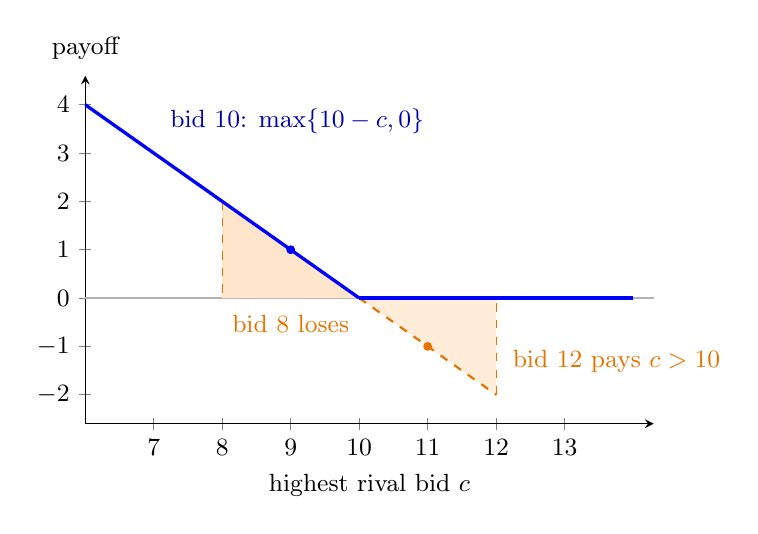
\begin{tikzpicture}[font=\small, >={Latex[length=2mm]}]
  \begin{axis}[
    axis lines=left, xmin=6, xmax=14.3, ymin=-2.6, ymax=4.6,
    xtick={7,8,9,10,11,12,13}, ytick={-2,-1,0,1,2,3,4},
    xlabel={highest rival bid $c$}, ylabel={payoff},
    ylabel style={rotate=-90, anchor=south, at={(axis description cs:0,1.02)}},
    width=8.8cm, height=6cm, clip=false]
    \addplot[gray!60, thin] coordinates {(6,0) (14.3,0)};
    % regions where the deviations differ from truthful bidding
    \addplot[fill=orange!20, draw=none] coordinates {(8,0) (8,2) (10,0)} -- cycle;
    \addplot[fill=orange!15, draw=none] coordinates {(10,0) (12,-2) (12,0)} -- cycle;
    % bid 12: follows 10 - c until c = 12
    \addplot[orange!90!black, thick, dashed, domain=10:12, samples=2] {10-x};
    \addplot[orange!90!black, thin, dashed] coordinates {(12,-2) (12,0)};
    % bid 8: drops to 0 at c = 8
    \addplot[orange!90!black, thin, dashed] coordinates {(8,2) (8,0)};
    % truthful bid 10
    \addplot[blue, very thick, domain=6:10, samples=2] {10-x};
    \addplot[blue, very thick] coordinates {(10,0) (14,0)};
    \fill[blue] (axis cs:9,1) circle (1.6pt);
    \fill[orange!90!black] (axis cs:11,-1) circle (1.6pt);
    \node[blue!70!black, anchor=south west] at (axis cs:7.1,3.2) {bid $10$: $\max\{10-c,0\}$};
    \node[orange!90!black, anchor=north] at (axis cs:9,-0.15) {bid $8$ loses};
    \node[orange!90!black, anchor=west] at (axis cs:12.1,-1.3) {bid $12$ pays $c>10$};
  \end{axis}
\end{tikzpicture}
\end{document}
